\section{Introduction}

% What we have done

% \begin{itemize}
%     \item Synthetic Data: We show how synthetic data can be generated for math domain
%     \item Reasoning: We generate it in conversational style to induce structure and complexity in reasoning. We think the conversational style helps with reasoning. \textbf{Potential missing experiment:} Rephrase the document vs conversational synthetic data generation [P1]
%     \item Comprehensive study on prompts: We experiment with 7 different prompt styles and pick the best one at 4B token scale
%     \item Scaling: We scale to pretraining 8B 300B and then scale it to 7B 1T token horizon. We also scale from 4B to 13B math tokens
%     \item \textbf{Extending to other math data:} We will show results on math-pile [P0], proof-pile
%     \item Potential to procure infinite math data: point of deepseekmath was that ``we gathered more and better data than owm". so we counter this and say we have a better methodology to get a lot more math data. Here we would have to show expts that compare with deepseekmath. We would need to generate more math data than what deepseekmath has and run expts. OR use all the syn data from all 7 prompts and do 7b 50B expt and then use the same number of tokens from original 4B owm [P3].
%     \item Quality control: We build a math quality classifier. Option 1: simply use finewebedu run inf. Option 2: we build a classifier using the same technique as finewebedu. Take \~100k samples and get scores for them using llama-3 or mistral nemo 12b. Then train a fasttext classifier on the scores [P2].
% \end{itemize}

% \begin{figure}[H]
%   \centering
%     \includegraphics[trim={0 0 0 0}, clip, width=1.0\columnwidth]{figures/intro_small.pdf}  
%   \caption{Continuous pretraining with synthetic math dialogues (\ourdata) results in improved mathematical and general purpose reasoning abilities of \llm compared to training with raw math corpus, \owm (\owma). Comparison between 3.6$\times$ large corpus (\owma-14B) and combination of different styles of conversations (\ourdata-4B) derived from a small subset (\owma-4B), reveals that model trained with combinations of conversations outperforms the one trained with larger corpus in \gsm, \mmlu and general reasoning---showing the significance of high-quality structured data over quantity.}
%   \label{fig:intro_img}
%   \vspace{-1mm}
% \end{figure}


% \shrimai{
% \begin{itemize}
%     \item Intro to LLMs and reasoning: LLMs have demonstrated remarkable performance across wide range of general purpose reasoning and specialized knowledge task
%     \item What is needed for such a reasoning: Strong mathematical reasoning needs high quality, composite and structured pretraining corpora. Moreover, solving complex reasoning problems, such as math questions, often requires breaking them down into smaller sub-problems. This step-by-step approach helps the model process and solve each component more effectively \citep{wei2022chain}, and has been widely adopted to improve few-shot reasoning during inference.
%     \item Problems: Curating such a data is costly and resource intensive. Curating such a dataset is not public info and such a pipeline / process is unclear. SDG has been used to curate such datasets. Most methods that curate such datasets don't care about breaking down into smaller problems.
%     \item To mitigate these challenges, we propose CONV-MATH method. Describe the method. Describe how it mitigates the above challenges.
%     \item In summary our contributions are: bullet point
%     \item Insights and numbers, results
% \end{itemize}
% }

The ability to reason is a fundamental element of human cognition, encompassing our ability to think logically, draw conclusions, and make decisions based on available information \citep{gendron2024large}. Large Language Models ({\llm}s) have demonstrated remarkable performance across wide range of general reasoning and specialized knowledge tasks. In particular, the improvement of {\llm}s in solving complex %and multi-hop 
mathematical reasoning tasks \citep{be83ab3e, cobbe2021gsm8k} has been significant in recent years \citep{geminiteam2024geminifamilyhighlycapable, 
%claude, 
nvidia2024nemotron4340btechnicalreport,openai2024gpt4technicalreport}.  

Strong mathematical reasoning ability heavily relies on the abundance of high-quality, composite, and structured pretraining corpora. %\shrimai{Potential Re-write: An effective mathematical corpus should not only contain relevant content but also be formatted to help models break down complex problems into smaller sub-problems, improving their ability to process and solve each step \citep{wei2022chain}.} %An effective mathematical corpus should not only contain relevant content but also be presented in a format that aligns with how models process and understand complex problems. Specifically, solving complex reasoning problems, such as math questions, often requires breaking them down into smaller sub-problems. This step-by-step approach helps the model process and solve each component more effectively \citep{wei2022chain}, and has been widely adopted to improve few-shot reasoning during inference.
An effective mathematical corpus should not only contain relevant content but also be formatted to guide models break down complex problems into smaller sub-problems and solve each part step-by-step---enhancing the model's ability to process and reason about complex problems \citep{wei2022chain}%---which has been widely adopted to improve few-shot reasoning during inference
. Prior studies show that structured and well-formatted corpora play a crucial role in enhancing multi-hop and logical reasoning abilities \citep{cobbe2021gsm8k, li2023textbooksneediiphi15, gunasekar2023textbooksneed}, underscoring the importance of well-organized mathematical datasets in pretraining {\llm}s.% add points about data not being in the correct format



Curating complex, high-quality structured mathematical data is costly and resource-intensive, largely due to the uneven distribution of high-quality sources.
Most advanced models \citep{openai2024gpt4technicalreport, geminiteam2024geminifamilyhighlycapable} are not publicly accessible, and it is unclear how their approach is enhancing math reasoning.
To mitigate this challenge, synthetic data generation has emerged as a scalable, and cost-effective alternative for creating a more balanced and diverse training corpus for pretraining {\llm}s \citep{rephrasing-the-web, eldan2023tinystoriessmalllanguagemodels, gunasekar2023textbooksneed, shah2024aiassistedgenerationdifficultmath}. 
%In fact, \cite{rephrasing-the-web} highlights that simply presenting raw data to models, without reformatting, is insufficient for improving reasoning abilities. While synthetic data has shown promise in improving general reasoning tasks, they often fall short in multi-hop reasoning and mathematical tasks \citep{rephrasing-the-web}. A key limitation is that current synthetic datasets fail to adopt a step-by-step reasoning structure crucial for solving complex problems. 
However, while these techniques have shown promise in improving general reasoning tasks, their data often lack the step-by-step problem solving structure crucial for multi-hop reasoning and complex mathematical tasks \citep{rephrasing-the-web}, making them sub-optimal for such reasoning.
%Although these structured synthetic datasets hold great potential for enhancing the complex reasoning abilities of {\llm}s, 
%However, curating pretraining-scale data of this nature from web is challenging and labour-intensive. 

%\shrimai{Re-write this to sound coherent. Say that existing SDG solutions don't focus on step-by-step approach. The data may not be in the format. Presenting the raw data to the model as is, is not enough.}

\begin{wrapfigure}[18]{r}{0.48\textwidth}
    \centering    
    \includegraphics[width=\textwidth]{figures/acc_size_color.pdf}
    \caption{Continuous pretraining with all styles of conversations (\ourdata-4B) derived from a small subset (\owma-4B) and a 3.6$\times$ large raw corpus (\owma-14B) reveals that model trained with conversations outperforms the one trained with larger corpus in \gsm, \mmlu and general reasoning---showing the significance of high-quality structured data over quantity.}
  \label{fig:intro_img}
  \vspace{-2mm}
\end{wrapfigure}

% To address these challenges, we propose \textbf{\ourapproach}, a novel approach to generate \textbf{M}ath \textbf{I}nformed sy\textbf{N}thetic \textbf{D}ialogue data at scale. In particular, we demonstrate that transforming raw web text into structured conversations using an off-the-shelf open-source \llm significantly enhances the mathematical and logical reasoning abilities of {\llm}s compared to relying on unstructured raw or rephrased web text. Additionally, relying on the web text to generate conversation provides us the flexibility to preserve diversity of the web corpora. As illustrated in \autoref{fig:conv_math}, \ourapproach generates conversation from a raw text by prompting an open-source \llm on seven diverse conversational styles. Building on prior observation that complex problem solving benefits from step-by-step breakdown of the problem, we explicitly prompt \llm to generate conversation that---(a) decompose the original context step-by-step into multi-turn conversations and (b) explore each step in depth within a single turn. Notably, the existence of knowledge imbalance between participants, whether explicit or implicit, in the conversation is crucial for further expansion of reasoning, as participants either educate each other or collaboratively bridge their shared knowledge gaps through explanation and analysis. The interactive and iterative nature of conversation allows for a continuous exchange of thoughts, where participants can build upon each other's thoughts, ask probing questions, and offer clarifications. Unlike static text rephrasing \citep{rephrasing-the-web}, conversations encourage dynamic reasoning, facilitating inclusion of complementary insights and explanations (As highlighted in the conversation of \autoref{fig:intro_img}). This quality makes conversations particularly effective for complex reasoning tasks, as they not only preserve the original information but also expand it with new layers of understanding and explanation. In summary, the key contributions of this work are as follows:


To address these challenges, we propose \textbf{\ourapproach}, a novel approach to generate \textbf{M}ath \textbf{I}nformed sy\textbf{N}thetic \textbf{D}ialogue data at scale. In \ourapproach, we provide a pretrained \llm with a web document and explicitly prompt it in a zero-shot manner to generate a conversation that---(a) decomposes the original context step-by-step into multi-turn conversations and (b) explores each step in depth within a single turn. As illustrated in \autoref{fig:conv_math}, \ourapproach generates conversation from a raw text by prompting an open-source \llm on seven diverse conversational styles. The generated conversations are refined using heuristic filters and then can be used to pretrain a language model.

\ourapproach demonstrates that transforming raw web text into structured conversations using an off-the-shelf open-source \llm significantly enhances the mathematical and logical reasoning abilities of {\llm}s compared to unstructured raw or rephrased web text. Additionally, \ourapproach provides the flexibility to preserve the diversity of the web corpora and leverage knowledge imbalances between participants for further expansion of the corpora as they either educate each other or collaboratively bridge their shared knowledge gaps through explanation and analysis in a conversation. Moreover, \ourapproach enables the continuous generation of synthetic data from a single document by employing infinite conversational styles, further enriching the diversity.
Unlike static text rephrasing \citep{rephrasing-the-web}, conversations encourage dynamic reasoning, where participants build on each other’s ideas, ask questions, and offer clarifications. This quality makes conversations particularly effective for complex reasoning tasks, as they not only preserve the original information but also expand it with new layers of understanding and explanation. %(As highlighted in the conversation of \autoref{fig:intro_img}). 

In summary, the key contributions of this work are as follows:


% \shrimai{
% To address these challenges, we propose \textbf{\ourapproach}, a novel approach to generate \textbf{M}ath \textbf{I}nformed sy\textbf{N}thetic \textbf{D}ialogue data at scale. 
% In the \ourapproach technique, we provide a pretrained \llm with a web document and explicitly prompt it in a zero-shot manner to generate conversation that---(a) decomposes the original context step-by-step into multi-turn conversations and (b) explores each step in depth within a single turn.
% As illustrated in \autoref{fig:conv_math}, \ourapproach generates conversation from a raw text by prompting an open-source \llm on seven diverse conversational styles. 
% The generated text is filtered using heuristic filters and then can be used to pretrain a language model.

% \ourapproach demonstrates that transforming raw web text into structured conversations using an off-the-shelf open-source \llm significantly enhances the mathematical and logical reasoning abilities of {\llm}s compared to unstructured raw or rephrased web text. 
% Additionally, \ourapproach provides us the flexibility to preserve diversity of the web corpora and to leverage knowledge imbalances between participants as they either educate each other or collaboratively bridge their shared knowledge gaps through explanation and analysis in a conversation. Unlike static text rephrasing \citep{rephrasing-the-web}, conversations encourage dynamic reasoning, where participants build on each other’s ideas, ask questions, and offer clarifications. This quality makes conversations particularly effective for complex reasoning tasks, as they not only preserve the original information but also expand it with new layers of understanding and explanation (As highlighted in the conversation of \autoref{fig:intro_img}). 

% In summary, the key contributions of this work are as follows:
% }

%\shrimai{Add the knowledge imbalance component.}
\begin{comment}
The ability to reason is a fundamental element of human cognition, encompassing our ability to think logically, draw conclusions, and make decisions based on available information \citep{gendron2024large}. Large Language Models ({\llm}s) have demonstrated remarkable performance across wide range of general purpose reasoning and specialized knowledge tasks. In particular, the improvement of {\llm}s in solving complex and multi-hop mathematical reasoning tasks \citep{be83ab3e, cobbe2021gsm8k} has been significant in recent years \citep{geminiteam2024geminifamilyhighlycapable, claude, openai2024gpt4technicalreport}.  However, most advanced models \citep{openai2024gpt4technicalreport, geminiteam2024geminifamilyhighlycapable} are not publicly accessible, and it is unclear how their approach is enhancing math reasoning. A major distinction between these cutting-edge models and publicly available ones lies in the scale and composition of the training data. Strong mathematical reasoning ability heavily relies on the abundance of high quality, composite and structured pretraining corpora. 
\end{comment}

%While some data curation approaches have been made public \citep{shao2024deepseekmathpushinglimitsmathematical, penedo2024finewebdatasetsdecantingweb, li2024datacomplmsearchgenerationtraining, NEURIPS2023_fa3ed726, deepseek-math}, majority of these data is still unstructured web content and very few of them specifically focuses on math reasoning. %Moreover, many of the most effective methods remain proprietary, with only limited information.

% To generate high-quality data at scale for pretraining, synthetic data generation approaches has gained prominence in recent times \citep{rephrasing-the-web, eldan2023tinystoriessmalllanguagemodels, gunasekar2023textbooks, shah2024aiassistedgenerationdifficultmath}. Curating complex and high quality structured mathematical data is expensive due to the skewed distribution of high quality data sources while synthetic data provides a feasible and inexpensive solution to create a balanced corpus. While recent synthetic data curation approaches improve the general reasoning tasks, they fall inadequate when assessing the performance of complex multi-hop reasoning and mathematical tasks \citep{rephrasing-the-web}. For mathematical reasoning, several works have shown the significance of synthetic math corpus in the paradigm of aligning pretrained {\llm}s via instruction fine-tuning, RLHF \citep{toshniwal2024openmathinstruct118millionmath, wang2024mathcoder, zeng2024skyworkmathdatascalinglaws}. However, these approaches introduce a significant ``knowledge bias" by selectively focusing on tasks that the model is intended to excel at making them inapplicable for curating diverse pretraining corpus. Although recent works try to address diversity through millions of persona \citep{chan2024scalingsyntheticdatacreation}, the question of how to evaluate the quality and ensure diversity when generating off-the-shelf synthetic mathematical data still remains \citep{yu2024large}.
\begin{comment}
Curating complex, high-quality structured mathematical data is costly and resource-intensive, largely due to the uneven distribution of high-quality sources. To mitigate this challenge, synthetic data generation has emerged as a scalable, and cost-effective alternative for creating a more balanced and diverse training corpus for pretraining {\llm}s \citep{rephrasing-the-web, eldan2023tinystoriessmalllanguagemodels, gunasekar2023textbooks, shah2024aiassistedgenerationdifficultmath}. %Synthetic data offers a practical and cost-effective alternative for creating a more balanced and diverse training corpus. 
However, while synthetic data has demonstrated success in improving general reasoning tasks, it often falls short in %complex, 
multi-hop reasoning and mathematical tasks \citep{rephrasing-the-web}. 
%Several studies have highlighted the importance of synthetic math corpora in aligning pretrained {\llm}s through instruction fine-tuning and RLHF \citep{toshniwal2024openmathinstruct118millionmath, wang2024mathcoder, zeng2024skyworkmathdatascalinglaws}. 
%However, these methods can introduce bias on tasks where the model is expected to excel, limiting their applicability in creating diverse pretraining corpora. 
%While some works attempt to address this by scaling synthetic data through millions of persona-driven prompts \citep{chan2024scalingsyntheticdatacreation} or by distilling skills from existing corpora \citep{shah2024aiassistedgenerationdifficultmath}, the challenges of evaluating quality and ensuring diversity in synthetic mathematical pretraining data generation remain unresolved \citep{yu2024large}.
%Strong mathematical reasoning needs high quality, composite and structured pretraining corpora. 
In addition, solving complex reasoning problems, such as math questions, often requires breaking them down into smaller sub-problems. This step-by-step approach helps the model process and solve each component more effectively \citep{wei2022chain}, and has been widely adopted to improve few-shot reasoning during inference. While these types of synthetic datasets hold great potential for enhancing the complex reasoning abilities of {\llm}s, curating pretraining-scale data of this nature from web is challenging. 
\end{comment}
% Generating large-scale synthetic mathematical data for pretraining presents a unique challenge. Unlike other domains, mathematical data requires precision, structure, and contextual relevance, where a small error in numbers, symbols, or steps could lead to significant inaccuracies.  


% \begin{figure}[H]
%   \centering
%     \includesvg[width=0.8\columnwidth]{figures/comp_data.svg}
%   \caption{Conversational synthetic data is better than simple rephrasing.}
%   \label{fig:comp_data}
% \end{figure}


% \begin{wrapfigure}{r}{0.5\textwidth}
%     \centering
%     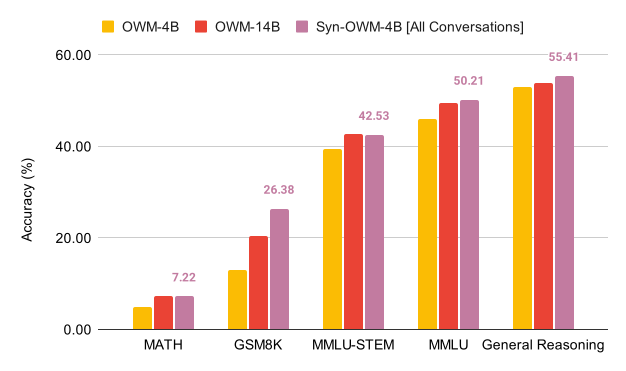
\includegraphics[trim={0 20 0 0}, clip, width=\textwidth]{figures/comp_data.pdf}
%     \caption{\label{fig:comp_data}}
% \end{wrapfigure}
\begin{comment}
In this work, we summarize the above observations in three key challenges associated with the generation and utilization of synthetic data for mathematical reasoning: (1) how to generate synthetic data to improve mathematical and logical reasoning ability when the underlying domain specific data is limited (2) how to engrave diversity in the generations and (3) how to ensure consistent improvement in math reasoning without hurting the performance of general purpose reasoning tasks. To address these challenges, we propose \textbf{\ourapproach}, a simple approach to generate \textbf{Conv}ersational Synthetic \textbf{Math} data at scale. In particular, we demonstrate that transforming raw web text into structured conversations using an off-the-shelf open-source \llm significantly enhances the mathematical and logical reasoning abilities of {\llm}s compared to relying on unstructured raw or rephrased web text. Additionally, relying on the web text to generate conversation provides us the flexibility to preserve diversity of the web corpora. Our approach generates conversations from a raw text by prompting an open-source \llm (\llama) on seven diverse conversational styles. 
\end{comment}

% \syeda{Add the numbers to the contributions}
\vspace{-2mm}
\begin{itemize}[leftmargin=*]
\itemsep0em
    \item We propose a novel approach, \ourapproach, to generate structured conversational synthetic data for math reasoning. Leveraging \ourapproach, we produce 64B tokens of synthetic data using 14B tokens from \owm corpus.
    % \item We have comprehensively experimented with different conversation styles by varying the roles of the participants for generating conversation and show a comparison between them. We provide this insight about the knowledge gap between two participants of a conversation to be a necessity in generating high quality math data.
    \item  We conduct comprehensive experiments with various conversational styles, altering participant roles to assess their impact on conversation quality and reasoning tasks. Our findings emphasize the importance of the knowledge imbalance between participants in producing high-quality mathematical data.
    % \item Additionally, we compare our approach with simple rephrasing of documents and chain of thought style of synthetic generation.
    \item We scale our approach to higher number of tokens and to two math specific datasets, demonstrating its efficacy in large and high-quality raw corpus.
    % \item Additionally, we provide insights into how the synthetic data and its combination with raw data should be provided during pretraining. \shrimai{Don't present the raw data as is. Rethink the data format.}
    \item %We demonstrate an effective way to integrate synthetic and raw data during pretraining that leads to a 6.29\% average improvement across three math benchmarks compared to raw data alone, emphasizing the importance of carefully reformatting raw data to optimize reasoning processes instead of using it in its original form.
    We demonstrate an effective way for integrating synthetic and raw data during pretraining to enhance mathematical reasoning ability of {\llm}s, emphasizing the importance of carefully reformatting raw data to optimize reasoning processes instead of using it in its original form. 
    % \item \shrimai{Check if we can release the data generated by llama 70B or 340B. Check if we can release the generation code and TRT-LLM pipeline.}
\end{itemize}
\vspace{-2mm}

% \shrimai{Improve this para, many confusing phrases.}
% In this paper, we evaluate \ourapproach across three dimensions: (1) the effectiveness of each conversational style in mathematical reasoning, (2) whether the impact of conversation persist as data scales, and (3) whether \ourapproach remains beneficial when the raw text originates from high-quality sources. When pretraining a 7B parameter \llm separately on a subset of \owm (\owma-4B) and synthetic conversations from \ourapproach (\ourdata-4B), the latter model achieves up to 6.29\% average improvement across three mathematical reasoning benchmarks, 4.30\% on specialized knowledge tasks (\mmlu), and a 2.20\% boost across 10 zero-shot tasks, compared to model trained with raw data. %In addition, our experiment using synthetic conversations on a single style generated from scaled raw data exhibits a consistent trend, demonstrating that conversational data enhances model performance even as datasets expand. 
In this paper, we evaluate \ourapproach across three dimensions: (1) the effectiveness of each conversational style in mathematical reasoning, (2) whether the impact of conversation persist as data scales, and (3) whether \ourapproach remains beneficial when the raw text originates from high-quality sources. Continuously pretraining a 7B \llm on synthetic conversations (\ourdata-4B), generated from a subset of \owm (\owma-4B), results in 6.29\% average improvement across three mathematical reasoning benchmarks, 4.30\% on specialized knowledge tasks (\mmlu), and a 2.20\% boost across 10 zero-shot tasks, compared to the model trained with raw \owma-4B. Additionally, our experiment with entire \owm (\owma-14B) and its corresponding synthetic conversations shows a consistent trend, indicating that the benefits of conversational data continue to hold as the data scales.
In fact, with all conversations generated from \owma-4B, we can outperform model trained with \owma-14B, a 3.6$\times$ larger data---2.94\% average improvement across \gsm and \mathall tasks, 1.56\% across all benchmarks (\autoref{fig:intro_img}). This underlines the value of synthetic conversations, particularly when high-quality in-domain data is limited. Moreover, our analysis with other datasets reveals that conversational data further amplifies reasoning capabilities in models even when the raw data originates from high-quality sources. We hope that \ourapproach will pave a way to improve complex reasoning ability of smaller models with limited training data and accelerate further innovation towards building strong reasoning ability with structured high-quality data.

%Ablations: (1) comparison with simple rephrasing (2) what is the best balance of raw and synthetic data (3) how to assess the quality of the generations. (4) ideal configuration for synthetic data generation


% This work aims to augment the reasoning ability of {\llm}s by generating conversational synthetic data that inherently requires deep comprehension of multi-hop scenarios and long context understanding. Our approach not only prepares a high-quality pretraining data for LLMs but also enhances the downstream reasoning tasks performance.
%Drawing the observation that complex problem solving benefits from step-by-step breakdown of the problem, we prompt 

% we introduce \ourapproach, a simple yet effective framework to generate synthetic mathematical data at scale for pretraining. In addition, solving complex reasoning problems such as math questions heavily benefits from breaking them down into smaller sub-problems step-by-step, enabling the model to process and tackle each component more effectively \citep{wei2022chain}.
 

%Additionally, synthetic data generation can introduce a significant ``knowledge bias" by selectively focusing on tasks that the model is intended to excel at. While synthetic data has demonstrated potential in improving performance \citep{rephrasing-the-web} during pretraining, it remains unclear whether this improvement stems from the inherently higher quality of synthetic data or from the deliberate choice of task-specific topics \citep{maini_phi_1_5}. 
    

%Yet they fall short when the underlying task demands complex and multi-hop logical reasoning specifically the mathematical reasoning tasks \citep{arora-etal-2023-llms, lu2023chameleon, he-etal-2024-olympiadbench, be83ab3e}.


% Distribution of high quality data sources is very skewed. Synthetic data can help create more balanced data sets.





% 1. We propose a novel synthetic data generation approach that goes beyond generating surface level linguistic variations and enhances raw text with semantic variations by adopting multi-hop conversational and reasoning format.
% 2. To promote diverse synthetic data generation at scale, this approach extends the synthesis across seven different conversational styles which steers the LLM towards the corresponding perspective to create distinctive synthetic data.